\documentclass[12pt,a4paper,oneside]{book}

\usepackage[utf8]{inputenc}
\usepackage{ucs}
\usepackage[english,russian]{babel}
\usepackage{extsizes} % чтобы можно было использовать шрифты больше, чем 12pt
\usepackage{pscyr} % красивые русскоязычные шрифты (мануал по установке тут: http://ishutov.blogspot.com/2011/02/miktex-29-pscyr-04d.html)
\usepackage{xcolor}
\usepackage{listings}
\usepackage{graphicx}
\usepackage{url}
\usepackage{lscape}

\usepackage{indentfirst}

% для математических символов
\usepackage{amsmath, amsthm, amssymb}

% для построения диаграмм
%\usepackage{tikz}
%\usetikzlibrary{positioning,arrows,shapes,shadows}

\lstset{inputencoding=utf8x}
\lstset{language=[Sharp]C}

\graphicspath{{pics/}}

% поля (в соответствии с Требованиями Оформления Магистерских Работ)
% по умолчанию левое и верхнее и левое поле = 1дюйм (2.54 см). Это соответствует требованиям.
\oddsidemargin = 0mm
\topmargin = -15mm % вычитается размер колонтитула.
\textwidth = 175mm
\textheight = 247mm

% абзацный отступ
\parindent = 12mm

\sloppy
\makeatletter
\renewcommand{\baselinestretch}{1.5} % межстрочный интервал

% чтобы каждая новая глава начиналась с новой страницы
\let\stdsection\section
\renewcommand\section{\newpage\stdsection}

\pagestyle{plain}

%\newcounter{appendix_number}
%\newcommand{\Appendix}[1]{\addtocounter{appendix_number}{1} \section{Приложение \arabic{appendix_number}. #1}}

% замена в подписи к рисунку разделителя ":" на "." (Рис. 2: Рисунок   станет   Рис. 2. Рисунок.) - - - - - - - - -
\renewcommand{\@makecaption}[2]{%
\vspace{\abovecaptionskip}%
\sbox{\@tempboxa}{#1: #2}
\ifdim \wd\@tempboxa >\hsize
#1: #2\par
\else
\global\@minipagefalse
\hbox to \hsize {\hfil #1. #2\hfil}%
\fi
\vspace{\belowcaptionskip}}
% - - - - - - - - - - - - - - - - - - - - - - - - - - - - - - - - - - - - - - - - - - - - - - - - - - - - - - - - - 


% - - - - - - - - - - - - - - - - - - - - - - - - - - - - - - - - - - - - - - - - - - - - - - - - - - - - - - - - - 
% оформление заголовков глав
 \def\onelineskip{\normalsize\vskip\baselineskip}

 \renewcommand{\@makechapterhead}[1]{%
 {\raggedright
 \parindent=0cm\hangafter=1%
 \newbox\numberbox
 \setbox\numberbox\hbox{\normalfont\LARGE\textar{\bfseries\thechapter.\hskip0.5em}}%
 \hangindent=\wd\numberbox %
 \normalfont\LARGE\textar{\@chapapp{}\bfseries
 \unhbox\numberbox #1}\par
 \nopagebreak
 \onelineskip
 }}

 \renewcommand{\@makeschapterhead}[1]{%
 {\parindent=0pt \raggedright
 \normalfont\LARGE\textar{\bfseries #1}\par
 \nopagebreak
 \onelineskip
 }}
% - - - - - - - - - - - - - - - - - - - - - - - - - - - - - - - - - - - - - - - - - - - - - - - - - - - - - - - - - 






\begin{document}
    %\renewcommand{\@oddhead}{\hfill \thepage \hfill} % номера страниц по центру сверху
    \renewcommand{\thesection}{\arabic{section}}
    \renewcommand{\bibname}{Источники}
    
    \newcommand{\TODO}[1]{\fcolorbox{red}{red}{TODO :: #1}}
    \newcommand{\Definition}[1]{{\bf Определение. } #1 \par} % TODO :: Добавить счётчик
   
    \setcounter{page}{4}   % номер первой страницы
	
    
    % Аннотация
	\setcounter{secnumdepth}{0}
\section*{Аннотация}
\setcounter{secnumdepth}{2}

При разработке современных программных комплексов зачастую возникают задачи, связанные с поддержкой функций расширения и автоматизации программного обеспечения. Это необходимо для реализации возможности конфигурирования, настройки, переопределения поведения, а также реализации недостоющего функционала приложения конечным пользователем. Чаще всего реализация данных возможностей достигается за счёт функций автоматического обновления программного обеспечения, поддержки плагинов сторонних производителей, наличия SDK (Software Development Kit) для разработки расширений, поддержки скриптов. С точки зрения числа предоставляемых возможностей и гибкости наибольший интерес представляет последний вариант. В зависимости от специфики разрабатываемого ПО могут быть различные сценарии использования скриптов: простейшее конфигурирование приложения конечным пользователем, разработка дополнений, расширяющих возможности приложения, распространение скриптов, разработанных сторонними производителями. В настоящее время многие разработчики предоставляют возможность использовать скрипты в своих приложениях. Помимо этого, существуют специальные технологии и платформы для интеграции скриптовых движков в приложения: VBA (Visual Basic for Applications), VSTA (Visual Studio Tools for Applications), VSTO (Visual Studio Tools for Office), IronPython, Game Maker Language) и другие. Основная проблема заклюается в том, чаще всего в каждом семействе программных продуктов разрабатываются собственные инструменты для интеграции поддержки скриптов в ПО. Существующие <<универсальные>> средства для решения этой задачи оказываются неэффективными и неудобными для использования на реальных проектах.

Целью данной работы является исследование существующих решений в области расширения и автоматизации ПО, а также создание универсальной платформы, включающей в себя инструменты для внедрения возможностей автоматизации и расширения в разрабатываемые программные продукты. Помимо самого механизма скриптов, разрабатываются утилиты для автоматического анализа кода основной программы и генерации вспомогательного кода. Платформа включает в себя механизм для отладки скриптов. Для достижения наибольшей эффектисности и охвата максимального числа сценариев использования в предложенном подходе объединяются возможности использования как интерпретируемых, так и компилируемых языков. 

На примере коммерческого проекта и проекта с открытым исходным кодом будут сравниваться возможности существующих продуктов и разработанной платформы. 
\pagebreak
	
	\tableofcontents
    \pagebreak
	
	% ---------  Основные главы -----------------------------------
	\setcounter{secnumdepth}{0} % за счёт этого "Введение" будет без номера
\section{Введение}
\setcounter{secnumdepth}{2}

Современное программное обеспечение (ПО) зачастую представляет из себя крупные программные комплексы, состоящие из множества различных компонентов. В процессе эксплуатации ПО одни компоненты могут устаревать, в других будут обнаружены критические ошибки и уязвимости. Помимо этого некоторым пользователям может оказаться необходим какой-то функционал, отсутствующий в базовой версии. Другие пользователи могут захотеть сконфигурировать приложение под свои нужды, автоматизировать некоторые его части. Все эти проблемы ведут к изучению вопросов, связанных с автоматизацией и расширением программного обеспечения.

Под {\it автоматизацией} программного продукта понимается возможность формировывать, сохранять и воспроизводить в автоматическом режиме некоторую последовательность пользовательских действий. К примеру, в популярном текстовом редакторе {\it Microsoft Word} для ускорения часто выполняемых операций редактирования или форматирования, а также для объединения нескольких команд или автоматизации обработки сложных последовательных действий в задачах можно записать макрос. В дальнейшем можно запускать этот макрос для повторения ранее записанных действий.

Под {\it расширением} программного приложения понимается возможность добавлять в существующий продукт новые модули, расширяющие возможности программы. Примером может служить популярный файловый менеджер {\it Far}, в который включён текстовый редактор. Однако в базовой конфигурации в редакторе нет подсветки синтаксиса языков программирования, в то время как многие разработчики используют его для написания кода. Недостоющий функционал добавляется за счёт планига (расширения) {\it Far Colorer}. 

Программное приложение, в дизайне которого предусмотрены возможности автоматизации и расширения, предоставет целый набор дополнительных преимуществ и для разработчика основного приложения, и для сторонних разработчиков, и для конечного пользователя:
\begin{itemize}
\item конфигурирование приложения конечным ползователем;
\item выпуск обновлённых и исправленных компонентов ПО;
\item разработка дополнений сторонними программистами;
\item автоматизация часто повторяющейся последовательности действий;
\item дополнение недостоющего функционала за счёт написания скриптов.
\end{itemize}

Раньше эти преимущества достигались за счёт периодических выпусков новых версий программного обеспечения. Это было не очень удобно, так как новые версии появлялись не так часто, и не было средств для решения проблем, содержащихся в текущей версии продукта. Был компромиссный вариант --- выпуск пакетов исправления ({\it Service Pack}) и пакетов новых возможностей ({\it Feature Pack}). 

Позже, с массовым распространением Интернета, этот подход был заменён автоматическим обнавлением. Суть осталась та же, только  пакеты исправлений и дополнений автоматически загружались с веб-сайта разработчика и автоматически устанавливались. 

Со временем, наряду с автоматическим обновлением, разработчики программного обеспечения стали добавлять в свои приложения возможности автоматизации и расширения. Этот шаг добавил программным комплексам большую гибкость, а также предоставил дополнительные возожности сторонним разработчикам. 

\pagebreak
	\section{Постановка задачи}
\label{sec:problem_statement}

Цель работы --- исследование вопросов, связанных с расширением и автоматизацией программного обеспечения, а также разработка и использование на реальном проекте платформы для интеграции поддержки возможностей расширения и автоматизации в .NET-приложения.

Данная задача возникла в рамках проекта по портированию приложения для управления инвестиционными портфелями с устаревших технологий на платформу {\it .NET}. В исходном приложении для интеграции возможностей автоматизации и расширения использовался набор инструментов {\it VBA}, включающий в себя скриптовый язык {\it VBA} и встроенную среду разработки {\it Visual Basic 6}. Так как {\it VBA} не совместима с платформой {\it .NET}, требовалась реализация платформы с аналогичными возможностями. 

Первоначальной задачей стал анализ исходного приложения, изучение сценариев его использования, в особенности функционала для создания и управления {\it VBA}-макросами. На основе сценариев использования были сформулированы требования к искомой платформе. Опираясь на эти требования, было проведено исследование рынка ПО и поиск продуктов с аналогичным или похожим функционалом, которое могло бы быть использовано в качестве полной или частичной замены {\it VBA} в портируемом приложении.

\subsection{Требования к платформе}
\label{sec:pl_requirements}

Платформа должна решать две основные задачи:
\begin{itemize}
 \item автоматизация ПО;
 \item расширение ПО.
\end{itemize}

В приложении, которое было разработано с использованием {\it VBA}, обе задачи решались за счёт возможности написания макросов на {\it Visual Basic}. Одни и те же макросы, в зависимости от контекста и конкретной задачи, могли как автоматизировать некоторые действия, так и расширять возможности приложения за счёт добавления нового функционала. Не было какого-то конкретного деления на <<автоматизацию>> и <<расширение>>. Поддержка макросов была реализована как некий отдельный модуль, тесно взаимодействующий с основным приложением, что было достаточно удобно и прозрачно для пользователя. Это и навело впервые на мысль рассматривать понятия автоматизации и расширения как одно целое (далее об этом речь пойдёт в разделе~\ref{sec:autom-and-ext-as-one-thing}).

\subsubsection{Сценарии использования}
Ниже будут описаны некоторые наиболее востребованные сценарии использования в соответствии с реальным проектом, о котором говорилось в разделе~\ref{sec:problem_statement}:
\begin{enumerate}
 \item реализация дополнительного формата импорта или экспорта данных. Ядро приложения предоставляет доступ к хранилищу данных и результатов вычислений. Помимо этого в приложении реализованы возможности экспорта и импорта в некоторых форматах. Однако иногда есть необходимость расширить набор форматов. Это можно сделать, реализовав соответствующий плагин с помощью разрабатываемой платформы;
 \item автоматизировать некоторую последовательность действий или вычислений, используя ядро приложения;
 \item добавить дополнительные диалоговые окна или элементы управления в существующий графический интерфейс пользователя, настроив таким образом приложение для конкретного пользователя;
 \item реализовать новый формат отчётов по инвестиционным портфелям в соответствии с требованиями конкретного пользователя.
\end{enumerate}

Приведённые формулировки сценариев использования довольно расплывчаты, более подробные формулировки потребовали бы углубления в детали проекта, что не имеет смысла в рамках данной главы. Однако из данных сценариев вытекают некоторые характеристики, которыми должна обладать платформа для автоматизации и расширения:
\begin{itemize}
 \item возможность контролируемого и безопасного доступа к данным приложения;
 \item возможность использования {\it API} основного приложения;
 \item возможность гибкой работы с кодом расширений --- для некоторых действий достаточно некоторого <<временного>> проекта-скрипта, который должен один раз выполниться и дальше будет невостребован, в то время как некоторые должны интегрироваться в приложение и использоваться при каждом его запуске, сохраняя возможность внесения изменений в код;
 \item возможность создания расширения сторонними разработчиками и распространения среди множества клиентов.
\end{itemize}

\subsubsection{Дополнительные возможности}
Рассмотрим некоторые дополнительные возможности, которыми могла бы обладать платформа для интеграции возможностей автоматизации и расширения в приложения. Такие возможности не являются первостепенными, но упрощают и ускоряют процесс интеграции в ПО, а также предоставляют дополнительный функционал конечным пользователям:

\begin{itemize}
\item автоматизированные инструменты для интеграции платформы в приложения. Могут включать в себя утилиты, которые анализируют код основного приложения, предоставляя пользователю информацию об общей структуре проекта и предлагая в полуавтоматическом режиме добавлять поддержку автоматизации и расширения (к примеру, за счёт генерации прокси-объектов);
\item предоставление инструментов, упрощающих написание кода скрипта в соответствии со специфичными особенностями конкретного приложения. Это может быть реализовано, к примеру, в виде усовершенствованного IntelliSense;
\item реализация контроля зависимостей расширений. В простейшем случае предполагается, что расширение зависит только от основного приложения. Однако в более сложном случае расширение может зависеть от других установленных в приложение расширений. Такие зависимости должны отслеживаться и удовлетворяться автоматически;
\item реализация централизованного хранилища расширений (репозитория). Сценарий использования такого репозитория следующий: разработчик крупного расширяемого программного комплекса размещает на своих серверах централизованный репозиторий поддерживаемых расширений. Расширения могут автоматически загружаться из приложения. Новые расширения могут добавляться в репозиторий как основным разработчиком приложения, так и сторонними разработчиками;
\item запись макроса (то есть последовательности пользовательских действий, выполненных с помощью графического интерфейса) и преобразование его в код.
\end{itemize}

\pagebreak


\pagebreak
	\subsection{Требования к платформе}
\label{sec:pl_requirements}

Платформа должна решать две основные задачи:
\begin{itemize}
 \item автоматизация ПО;
 \item расширение ПО.
\end{itemize}

В приложении, которое было разработано с использованием {\it VBA}, обе задачи решались за счёт возможности написания макросов на {\it Visual Basic}. Одни и те же макросы, в зависимости от контекста и конкретной задачи, могли как автоматизировать некоторые действия, так и расширять возможности приложения за счёт добавления нового функционала. Не было какого-то конкретного деления на <<автоматизацию>> и <<расширение>>. Поддержка макросов была реализована как некий отдельный модуль, тесно взаимодействующий с основным приложением, что было достаточно удобно и прозрачно для пользователя. Это и навело впервые на мысль рассматривать понятия автоматизации и расширения как одно целое (далее об этом речь пойдёт в разделе~\ref{sec:autom-and-ext-as-one-thing}).

\subsubsection{Сценарии использования}
Ниже будут описаны некоторые наиболее востребованные сценарии использования в соответствии с реальным проектом, о котором говорилось в разделе~\ref{sec:problem_statement}:
\begin{enumerate}
 \item реализация дополнительного формата импорта или экспорта данных. Ядро приложения предоставляет доступ к хранилищу данных и результатов вычислений. Помимо этого в приложении реализованы возможности экспорта и импорта в некоторых форматах. Однако иногда есть необходимость расширить набор форматов. Это можно сделать, реализовав соответствующий плагин с помощью разрабатываемой платформы;
 \item автоматизировать некоторую последовательность действий или вычислений, используя ядро приложения;
 \item добавить дополнительные диалоговые окна или элементы управления в существующий графический интерфейс пользователя, настроив таким образом приложение для конкретного пользователя;
 \item реализовать новый формат отчётов по инвестиционным портфелям в соответствии с требованиями конкретного пользователя.
\end{enumerate}

Приведённые формулировки сценариев использования довольно расплывчаты, более подробные формулировки потребовали бы углубления в детали проекта, что не имеет смысла в рамках данной главы. Однако из данных сценариев вытекают некоторые характеристики, которыми должна обладать платформа для автоматизации и расширения:
\begin{itemize}
 \item возможность контролируемого и безопасного доступа к данным приложения;
 \item возможность использования {\it API} основного приложения;
 \item возможность гибкой работы с кодом расширений --- для некоторых действий достаточно некоторого <<временного>> проекта-скрипта, который должен один раз выполниться и дальше будет невостребован, в то время как некоторые должны интегрироваться в приложение и использоваться при каждом его запуске, сохраняя возможность внесения изменений в код;
 \item возможность создания расширения сторонними разработчиками и распространения среди множества клиентов.
\end{itemize}

\subsubsection{Дополнительные возможности}
Рассмотрим некоторые дополнительные возможности, которыми могла бы обладать платформа для интеграции возможностей автоматизации и расширения в приложения. Такие возможности не являются первостепенными, но упрощают и ускоряют процесс интеграции в ПО, а также предоставляют дополнительный функционал конечным пользователям:

\begin{itemize}
\item автоматизированные инструменты для интеграции платформы в приложения. Могут включать в себя утилиты, которые анализируют код основного приложения, предоставляя пользователю информацию об общей структуре проекта и предлагая в полуавтоматическом режиме добавлять поддержку автоматизации и расширения (к примеру, за счёт генерации прокси-объектов);
\item предоставление инструментов, упрощающих написание кода скрипта в соответствии со специфичными особенностями конкретного приложения. Это может быть реализовано, к примеру, в виде усовершенствованного IntelliSense;
\item реализация контроля зависимостей расширений. В простейшем случае предполагается, что расширение зависит только от основного приложения. Однако в более сложном случае расширение может зависеть от других установленных в приложение расширений. Такие зависимости должны отслеживаться и удовлетворяться автоматически;
\item реализация централизованного хранилища расширений (репозитория). Сценарий использования такого репозитория следующий: разработчик крупного расширяемого программного комплекса размещает на своих серверах централизованный репозиторий поддерживаемых расширений. Расширения могут автоматически загружаться из приложения. Новые расширения могут добавляться в репозиторий как основным разработчиком приложения, так и сторонними разработчиками;
\item запись макроса (то есть последовательности пользовательских действий, выполненных с помощью графического интерфейса) и преобразование его в код.
\end{itemize}

\pagebreak

	\section{Существующие решения}

\subsubsection{Visual Basic for Applications}

{\it Visual Basic for Applications} -- разработка компании {\it Microsoft}, совмещающая в себе реализацию языка программирования {\it Visual Basic} и соответствующую среду разработки~\cite{mastering-vba}. {\it VBA} является интерпретируемым языком: исходный код программы компилируется в промежуточный {\it P-код}, который впоследствии выполняется виртуальной машиной, являющейся частью основного приложения. {\it VBA} построен на технологии {\it COM}, благодаря чему {\it VBA-}код может использовать все доступные в операционной системе {\it COM}-объекты и компоненты {\it ActiveX}. Интегрированная среда разработки предоставляет удобный редактор кода с подсветкой синтаксиса и системой автодополнения кода, набор инструментов для удобной работы с проектами и файлами исходного кода, а также отладчик. Одно из важных достоинств {\it VBA} -- сравнительная лёгкость освоения.

Изначально {\it VBA} был встроен в семейство продуктов {\it Microsoft Office}. Из кода макроса на {\it VBA} пользователь может получить доступ ко всем функциям, доступным через графический интерфейс пользователя, а также к многочисленным функциям операционной системы и компонентов сторонних разработчиков.

Помимо {\it Microsoft Office} {\it VBA} встроен во многие программные продукты других разработчиков, к примеру,  {\it AutoCAD}, {\it SolidWorks}, {\it CorelDRAW}, {\it WordPerfect} и {\it ESRI ArcGIS}. Более того, {\it VBA} можно использовать при разработке любого {\it Windows}-приложения для внедрения в него возможности автоматизации. 

В настоящее время технология {\it VBA} считается устаревшей и более не поддерживается. В качестве замены {\it Microsoft} предлагает технологии {\it VSTA}~\cite{vsta-website} и {\it VSTO}~\cite{vsto-website}, речь о которых пойдёт в следующих разделах.
\subsection{Visual Studio Tools for Applications}

{\it Visual Studio Tools for Applications (VSTA)} -- это набор инструментов, который независимые поставщики программного обеспечения могут использовать для добавления возможностей автоматизации и расширения в свои приложения. {\it VSTA} был объявлен {\it Microsoft} с выпуском интегрированной реды разработки {\it Visual Studio 2005}. {\it VSTA} основана на платформе {\it .NET Framework} и построена на той же архитектуре, что и {\it VSTO}, речь о которой пойдёт в следующем разделе. {\it VSTA} включает в себя интегрированную среду разработки, являющуюся упрощённой версией IDE {\it Visual Studio}. Основные языки программирования, используемые в {\it VSTA} -- это {\it Visual Basic .NET} и {\it C\#}, однако в общем случае может быть использован любой язык для платформы {\it .NET}. Благодаря тесной интеграции с {\it .NET} пользовательский код имеет доступ ко всей библиотеке классов этой платформы, что существенно расширяет спектр возможностей при написании расширений и макросов. Важной особенностью {\it VSTA} является поддержка 64-битной архитектуры. 

Платформа {\it VSTA} распространется бесплатно, однако разработчики, планирующие включать {\it VSTA} в состав коммерческого приложения, должны приобрести соответствующую лицензию.
\subsubsection{Visual Studio Tools for Office}

{\it Visual Studio Tools for Office} -- это набор средств разработки, доступных в виде расширений {\it Visual Studio} (шаблонов проектов) и исполняющей среды, позволяющей  семейству продуктов {\it Microsoft Office} 2003 и более поздних версий загружать и выполнять пользовательский код {\it .NET} для расширения функциональности приложений {\it Office} и их автоматизации~\cite{vsto-website}. {\it VSTO} пришла на замену технологии {\it VBA}, использующейся в более ранних версиях {\it Microsoft Office}. 

Расширения {\it VSTO} разрабатываются в интегрированной среде {\it Visual Studio}. Пользовательский код имеет доступ ко всей библиотеке классов {\it .NET}. Как и в случае с {\it VBA}, макрос выполняется виртуальной машиной (в данном случае - CLR, Common Language Runtime), которая работает в рамках процесса основного приложения. Но в отличие от {\it VBA} код сохраняется в отдельной сборке {\it .NET}.

\pagebreak
	\section{Теоретическое исследование}

\subsection{Расширяемость и автоматизация как единое понятие}
\label{sec:autom-and-ext-as-one-thing}

Во введении были даны определения расширяемости и автоматизации программного обеспечения. С одной стороны, эти два понятия имеют мало общего и могут существовать раздельно. Действительно, программный продукт может предоставлять возможность использовать скрипты для автоматизации, но не поддерживать плагины-расширения. Или наоборот, для приложения может быть разработана развитая система плагинов с автоматическим контролем и обновлением версий, с удобным <<магазином>> расширений, но поддержка автоматизации может отсутствовать.

Как будет показано далее, некоторые существующие решения для интеграции возможностей автоматизации и расширяемости поддерживают сразу оба механизма, некоторые --- только что-то одно. Этому есть объяснение. В некоторых случаях нет необходимости реализовывать оба подхода. Этот вывод подтверждается практикой --- многие современные приложения поддерживают либо автоматизацию, либо расширения, и этого бывает достаточно. Но, как говорилось во введении, данные вопросы встают более остро в крупных программных комплексах, состоящих из множества компонентов. В таких ситуациях зачастую актуальны оба понятия. В связи с этим был сделан вывод о том, что понятия автоматизации и расширяемости можно рассматривать как одно целое. Более того, если это учесть при дизайне приложения, реализовывать поддержку этих механизмов также можно совместно и сделать их неразделимыми.




Для написания пользовательских расширений могут использоваться как скрипты (в терминологии некоторых программ «макросы»)~\cite{automata-via-macros}, так и плагины (независимые модули, написанные на компилируемых языках)~\cite{addins-and-extensibility}.

\subsubsection{Скриптовый язык удобен в следующих случаях:}

\begin{enumerate}
\item Если нужно обеспечить программируемость без риска дестабилизировать систему. Так как, в отличие от плагинов, скрипты интерпретируются, а не компилируются, неправильно написанный скрипт выведет диагностическое сообщение, а не приведёт к системному краху;
\item Если важен выразительный код. Во-первых, чем сложнее система, тем больше кода приходится писать «потому, что это нужно. Во-вторых, в скриптовом языке может быть совсем другая концепция программирования, чем в основной программе — например, игра может быть монолитным однопоточным приложением, в то время как управляющие персонажами скрипты выполняются параллельно. В-третьих, скриптовый язык имеет собственный проблемно-ориентированный набор команд, и одна строка скрипта может делать то же, что несколько десятков строк на традиционном языке. Как следствие, на скриптовом языке может писать программист очень низкой квалификации — например, дизайнер своими руками, не полагаясь на программистов, может корректировать правила игры;
\item Если требуется кроссплатформенность. Хорошим примером является JavaScript — его исполняют браузеры под самыми разными ОС.
\end{enumerate}

\subsubsection{У плагинов же есть три важных преимущества:}

\begin{enumerate}
\item Готовые программы, оттранслированные в машинный код, выполняются значительно быстрее скриптов, которые интерпретируются из исходного кода динамически при каждом исполнении. Поэтому скриптовые языки не применяются для написания программ, требующих оптимальности и быстроты исполнения. Но из-за простоты они часто применяются для написания небольших, одноразовых («проблемных») программ;
\item Полный доступ к любому аппаратному обеспечению или ресурсу ОС (в скриптовом языке для этого должен существовать написанный на машинном коде API). Плагины, работающие с аппаратным обеспечением, традиционно называют драйверами;
\item Если предполагается интенсивный обмен данными между основной программой и пользовательским расширением, для плагина его обеспечить проще.
\end{enumerate}

Также в плане быстродействия скриптовые языки можно разделить на языки динамического разбора (sh) и предварительно компилируемые (perl). Языки динамического разбора считывают инструкции из файла программы минимально требующимися блоками, и исполняют эти блоки, не читая дальнейший код. Предкомпилируемые языки транслируют всю программу в байт-код и затем исполняют его. Некоторые скриптовые языки имеют возможность компиляции программы «на лету» в машинный код (т. н. JIT-компиляция).

\subsection{Формулировка задачи}

В рамках портирования с COM на .NET крупного приложения для управления инвестиционными портфелями потребовалось замена технологии VBA на аналогичною .NET совместимую технологию. Таким образом, потребовалось провести исследование рынка ПО и поиск продуктов с аналогичным или похожим функционалом.

\subsubsection{Основные требования к программному продукту}

\begin{enumerate}
\item Возможность создания расширений для конечных пользователей;
\item Простота использования (Не требует SDK и другого ПО для создания расширений. Вся работа происходит в среде разработки (IDE));
\item Возможность работы как под x86, так и под x64 архитектурами;
\item Возможность отладки расширения;
\item Доступ расширения к объектам расширяемого приложения, реакция на его события;
\item При изменении удалении или добавлении объекта в хост приложении, расширение должно автоматически обновлять информацию о своем окружении;
\item Доступ к библиотеке классов .NET Framework;
\item Поддержка большого числа расширений и взаимодействие их друг с другом;
\item Возможность разрешения зависимостей между расширениями;
\item Удобные инструменты для написания кода (Аналогично инструментам IntelliSense в Microsoft Visual Studio);
\item Возможность сохранения расширений по усмотрению пользователя в базу данных, архив, папку и т. д.;
\item Динамическая загрузка и выгрузка расширений из адресного пространства хост приложения;
\item Компиляция и перезагрузка расширения «на лету» (Не требуется перезапуск хост приложения).
\end{enumerate}

\subsection{Применимость существующих решений}
\paragraph{VBA}
\paragraph{VSTA}
\paragraph{VSTO}


\subsection{Разработка новой платформы для решения поставленной задачи}

\pagebreak
	
\section{Перечень задач}

\subsection{Интеграция со средой разработки}

Один из важнейших сценариев использования расширяемых и автоматизируемых программных продуктов --- возможность разработки новых скриптов и редактирование кода старых в интегрированной среде разработки.

Встроенная среда разработки как правило поставляется вместе с продуктами для автоматизации приложений, например VBA или VSTA. В платформах, основная цель которых --- поддержка плагинов, напротив, встроенных средств для редактирования кода не предоставляется. Это понятно, так как считается, что конечный пользователь не будет заниматься такой сложной задачей, как написание расширения к своему приложению. Для разработчиков же существуют отдельные пакеты (SDK) для разработки расширений в различных средах разработки.

При реализации платформы для автоматизации и расширения необходимо было предоставить удобные средства редактирования кода конечному пользователю. Эта задача может быть решена несколькими способами:

\subsubsection{Реализация собственного редактора исходного кода расширений}

Это решение имеет как и преимущества, так и целый ряд существенных недостатков. Положительным моментом этого подхода является простота интеграции в разрабатываемую платфому. Однако, реализация действительно удобного набора инструментов, таких как подсветка синтаксиса, автодополнение, автогенерация кода по шаблонам, управления файлами с исходным кодом, будет очень сложной задачей. Кроме того, результат в любом случае наврядли сравниться с современными IDE.

\subsubsection{Использование одной из существующих IDE}

Это решение хорошо тем, что мы получаем готовую среду разработки с множеством встроенных инструментов. Одноко, встает ряд вопросов, которые необходимо решить для успешного применения сторонней IDE в разрабатываемой платформе.

Интеграция в платформу. Под интеграцией необходимо понимать возможность программного управления сторонней IDE на уровне, достаточном для того, чтобы у пользователя складывалось ощущение, что он работает с единой системой, а не несколькими разными программами.

Большинство IDE обладают куда более широким, чем нужно для разработки расширений, функционалом. Поэтому важным критерием выбора сторонней IDE является ее настраиваемость и конфигурируемость. Это касается как доступных пользователю функций, так и внешного вида самой среды.

Несмотря на предыдущий пункт, в котором сказано, что функционал современных сред разработки излишен для использования их в качастве редактора расширений, может случиться так, что некоторых специфичных функций будет нехватать. Поэтому искомая среда должна также обладать возможностью расширения функционала. Отдельным плюсом будет поддержка плагинов. Тогда можно будет отключать ненужные плагины и разработать плагины, добавляющие новый функционал.

Рассмотрим существующие среды разработки под платформу .NET.

\subsubsection{MS Visual Studio}

Удобная и мощная среда разработки от компании Microsoft. Распространяется в нескольких редакциях, различных по стоимости и функционалу. Помимо платных Professional и Ultimate версий существует бесплатная Express редакция.

Эта IDE поддерживает плагины, и имеет огромное количество разнообразных расширений, повышающих эффективность разработки.

Так же она поддерживает довольно гибкий механихм пользовательских настроек, что позволяет разработчику настроить ее <<под себя>>. Однако, отключить ненужные функции этот механизм не позволяет.

Поддерживает программное управление благодаря наличию  DTE --- объекта верхнего уровня в объектной модели автоматизации Visual Studio. Этот объект используется для доступа к функциональности. Доступ к этому объекту осуществляется через EnvDTE — это обернутая сборка COM-библиотеки, содержащая объекты и члены для автоматизации ядра Visual Studio. При помощи DTE можно программно управлять средой разработки, переопределять ее поведение. Таким образом Visual Studio может быть интегрирована в платформу.

Стоит отметить, что использование DTE для управления бесплатной версией Visual Studio Express невозможно, так как в ней отсутствуют необходимые для этого компоненты.

\subsubsection{SharpDevelop}

SharpDevelop — свободная среда разработки для C\#, Visual Basic .NET, Boo, IronPython, IronRuby, F\#, C++. Обычно используется теми, кто не хочет пользоваться Visual Studio .NET.

SharpDevelop предоставляет интегрированный отладчик, который использует собственные библиотеки и взаимодействует с исполняющей средой .NET через COM Interop.

У этой среды разработки есть ряд особенностей и преимуществ:

Во-первых, эта IDE может управляться программно извне при помощи встроенной технологии SDA (SharpDevelop for Applications). Программное управление позволяет выполнять различные действия в IDE без участия пользователя. Например, показывать или скрывать само приложение, запускать сборку проекта, управлять сохранением и загрузкой проектов, и многие другие. 

Во-вторых, эта IDE поддерживает плагины. Это свойство позволит добавить какую-либо отсутствующую в базовой поставке функциональность не меняя исходного кода самого SharpDevelop. Это важно, так как изменение исходного кода сделает неудобным распространение готовой платформы, так как она будет совместима только с конкретной сборкой SharpDevelop. Использование плагинов позволит добавить нужную функцинальность в уже установленный экземпляр этой IDE.

В-третьих, SharpDevelop поддерживает кастомизацию, то есть изменение своего внешного вида и поведения при момощи конфигурационных файлов. Под изменением внешнего вида нужно понимать удаление <<лишних>> в контексте данного сценария использования (как внешней IDE для разработки расширений) элементов управления, добавление новых элементов управления, управление доступностью этих элементов, и прочее. Изменение поведения состоит в подмене штатных обработчиков событий элементов управления (например, кнопок), на свои собственные обработчики с измененной логикой. Например, запуск отладчика не должен пытаться стартовать сборку самого расширения (это попросту невозможно, так как расширения представляет из себя библиотеку классов), а присоединить отладчик к процессу хост-приложения.

В-четвертых, открытый исходных код поможет быстрее решить проблемы, связанные с интеграцией SharpDevelop в разрабатываемую платформу. Код IDE может быть отредактирован благодаря открытой лиценции GNU GPL v2. IDE может быть запущена под отладчиком для выявления и локализации проблем вызванных внешними факторами и нетипичным использованием самой IDE.

Наконец, она распространяется бесплатно, что делает ее очень привлекательным выбором для использования в разрабатываемой платформе.

Из недостатков этой среды стоит отметить не такой богатый инструментарий, как в VisualStudio, отсутствие аналогов многих полулярных в сообществе .NET-разработчиков в среде  VisualStudio планинов, таких как ReSharper. Не такой удобный редактор исходного кода и визуальных элементов. С другой стороны, SharpDevelop не такой <<тяжеловесный>> и потребляет мало ресурсов, что немаловажный фактор в предполагаемом сценарии его использования, как внешней среды для редактирования исходного кода расширений.

\subsubsection{MonoDevelop}

Этот продукт является кроссплатформенным форком, то есть клоном SharpDevelop, и имеет сходный с ним функционал. Более подробно рассматривать ее не имеет большого смысла. Все плюсы и минусы SharpDevelop имеют отношение и к MonoDevelop. Однако, MonoDevelop не поддерживает программное управление, в отличие от SharpDevelop, что делает SharpDevelop более предпочтительным выбором для решения поставленной задачи.

\subsubsection{Вывод}

В качестве внешней IDE для разработки расширений была выбрана IDE с открытым исходным кодом SharpDevelop. Помимо того, что она распространяется бесплатно, имеет открытый исходный код и потребляет меньше ресурсов системы под свои нужды, инсталляционный пакет SharpDevelop имеет куда меньшие размеры, чем Visual Studio, и не содержит такое многообразие различных компонент, которые будут лишними на рабочей станции рядового пользователя ПО (не разработчика).

\pagebreak

\subsection{Меж-процессное взаимодействие}

\TODO{обзор возможных технологий, выводы}

\pagebreak

\subsection{Интеграция расширений}
\label{sec:extention_interaction}

\TODO{обзор возможных технологий, выводы}

\pagebreak

\subsection{Интеграция в расширяемое приложение}
\label{sec:app-integration}

Задачу интеграции разрабатываемой платформы можно разделить на два случая:

\begin{itemize}
  \item интеграция в готовое приложение;
  \item интеграция в приложение на этапе разработки.
\end{itemize}

Задача интеграции платформы в разрабатывоемое приложение не вызывает затруднений как для платформы, описываемой в работе, так и для большинства рассмотреных аналогов, так как на этом этапе программист имеет возможность продумать архитектуру приложения с учетом использования того или иного решения для интеграции возможностей автоматизации и/или расширения. Сложность интеграции в этом случае в большей степени зависит от решений, принятых разработчиком, чем от принципов, заложенных в интегрируемом продукте. Безусловно, лубой продукт требует наличия опыта работы с ним для получения лучших результатов.

Куда более интересна задача интеграции платформы в приложение, код которого уже написан, и архитектура не потерпит изменений. В этом случае большинство из существующих решений оказывабтся настолько сложны в интеграции из-за особенностей своего внутреннего устройства, что можно заявлять, что для этих продуктов такая задача будет практически неразрешимой. Все дело в сложности принципов построения взаимодействия между расширением и приложением, заложенных в большинстве существующих решений. Эти принципы сложны, потому что преследуют цели полной изоляции приложения от расширения, создания универсальных механизмов взаимодействия, а так же из-за использования тех или иных шаблонов проектирования. Этот факт не делает существующие решения плохими, наоборот, все решения, используемые в этих продуктах имеют серьёзное теоретическое обоснование, диктуемое принципапи проектирования программного обеспечения, но, к сожалению, из-за этого применение существующих решений в рамках интеграции возможностей расширения в существующее приложение становиться очень трудоёмкой задачей.

В работе стояла именно задача интеграции разрабатываемой платформы в уже существующее приложение. Опираясь на результаты, полученные в предыдущих разделах, решение этой задаци состоит из нескольких этапов:

\begin{itemize}
  \item выделение в коде приложения типов, объекты которых должны быть доступны со стороны расширения;
  \item реализация этими классами интерфейса, предаставляемого модулем платформы, отвечающим за взаимодействие с расширениями;
  \item создание классов-наблюдателей, храшящих список объектов одного типа, и реагирующих на все изменения количества и состояния этих объектов;
  \item регистрация этих классов-наблюдателей в модуле поддержки взаимодействия с расширениями;
  \item внедрение пользовательских элементов управления расширениями, предоставляемых платформой.
\end{itemize}

\pagebreak


\pagebreak


\subsection{Архитектура платформы}
\label{sec:fw_arch}

В этом разделе будет рассмотрена укрупненная схема архитектуры платформы; расположение и назначение компонентов системы и их взаимодействие.

После определения спектра глобальных задач, подлежащих решению в рамках реализации платформы, и выбора используемых для их решения технологий, инструментов и подходов, а также учитывая опыт существующих разработок, направленных на решение поставленной задачи, в особенности {\it VBA} и {\it VSTA}, была разработана концептуальная модель взаимодействия основных компонентов платформы~\cite{patterns-of-enterprise-app}.

Как видно на рисунке \ref{fw_arch1}, система состоит из двух отдельных процессов. Такая архитектура обусловлена необходимостью поддержку отладки расширений, а отладчик, как известно, должен выполняться в отдельном процессе. Кроме того, хост-процесс IDE является дочерним для процесса хост-приложения. Управление этими процессами организовано таким образом, что в случае прекращения из-за критической ошибки работы процесса, обслуживающего IDE, этот процесс будет автоматически перезапущен. В таком случае система продолжит работу в штатном режиме. Напротив, при сбое в процессе хост-приложения, будет остановлен так же хост-процесс IDE, что позволяет предотвратить возникновения в системе <<паразитных>> процессов.

Согласно разделу \ref{sec:ide-integration}, в качестве внешней среду разработки была выбрана свободная среда разработки с открытым исходным кодом SharpDevelop. Более того, благодаря совместимости библиотек входящих в состав этой IDE, реализована поддержка версий SharpDevelop 3.2 и 4.1, а так же не исключается возможность поддержки последующих версий. Таким образом, реализуемая платформа может быть с успехом использована в приложениях, реализованных на различных версиях платформы .NET. Для временного хранения managed-сборок расширений, компилируемых средой разработки, используется изолированное хранилище. Подробнее про управление сборками расширений написано в разделе \ref{sec:dll_manip}.

\begin{figure}[!h]
    \centering
    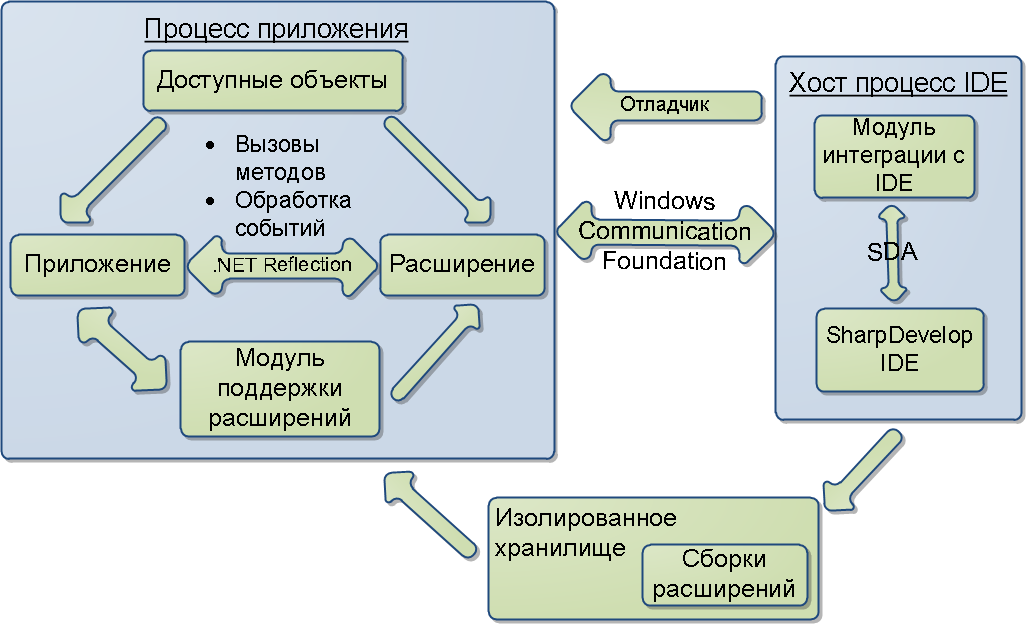
\includegraphics[width=15cm]{fw_arch1_fixed.png}
    \caption{Взаимодействие компонентов системы}
    \label{fw_arch1}
\end{figure}

Межпроцессное взаимодействие в разрабатываемой системе было решено реализовать при помощи именованных каналов {\tt (named pipe)} из библиотеки WCF (Windows Communication Foundation)~\cite{wcf-services}. Выбор WCF обусловлен тем, что эта библиотека входит в состав .NET Framework, и использование ее будет наиболее оправдано для разработки приложения под эту платформу. Реализация именнованых каналов в WCF --- NetNamedPipe, выбрана по причине того, что в рамках решения задачи по обеспечению взаимодействия двух процессов на локальной машине нет необходимости в использовании более сложных и емких механизмов взаимодействия, чем именованные каналы. Подробнее особенности реализации межпроцессного взаимодействия были рассмотрены ранее в разделе~\ref{sec:ipc}.

Взаимодействие между процессами происходит по двум отдельным именованным каналам, так как инициировать запросы (то есть выступать в роли сервера) могут оба процесса, и механизм <<запрос --- ответ>> в данном случае не подходит.

Более того, адреса, по которым взаимодействуют процессы выбираются случайно, что позволяет без возникновения конфликтов запускать множество пар процессов <<приложение --- IDE>>. Такое решение позволит использовать разрабатываемую платформу в нескольких приложениях одновременно.

Для работы с расширениями и IDE в приложение должен быть интегрирован специальный модуль, выполняющий сервисные задачи по обеспечению взаимодействия расширения с приложением, приложения с хост-процессом IDE, а так же предоставляющий пользователю набор визуальных компонент для управления системой. Этот модуль показан на рисунке \ref{fw_arch1} (Модуль поддержки расширений). Его назначение и особенности разработки будут описаны далее.

Взаимодействие расширения и приложения реализовано через {\it .NET Reflection}~\cite{cs2008-dotnet35}, как описано в разделе~\ref{sec:extention_interaction}. Взаимодействие осуществляется через динамическое привязывание к доступным объектам приложения, которые должны подчиняться определенным <<правилам игры>>, чтобы быть доступными для расширения. Выделение видимых объектов и создание уровня доступа к ним --- главная задача интеграции платформы в готовое приложение. Подробнее особенности интеграции разрабатываемой платформы были рассмотрены в разделе~\ref{sec:app-integration}.

\subsection{Применение разработанной платформы на существующем Open-Source проекте}

\TODO{Да, я искренне в это верю!}

\pagebreak

	\section{Сравнение с аналогами}

Единственным непосредственным аналогом разработанной платформы является VSTA. (речь идет о ПО для платформы .NET)  Сравнение будет происходить основываясь на опыте применения технологии VSTA в реальном проекте (см раздел \ref{sec:use_exis_techn}). Кроме того, в рамках данной работы необходимо оценить успешнось разработанной платформы, как замены устаревшего инструментария VBA, так как один из сценариев применения платформы - замена VBA при портировании COM/ActveX-приложений, использующих VBA, на платформу .NET.

\subsubsection{Методика сравнительного анализа}

Рассматриваемые плаформы поддержки расширений можно представить как совокупность следующих компонент:

\begin{itemize}
   \item среда разработки расширений;
   \item пользовательский интерфайс (инструментарий для работы с расширениями);
   \item ядро, обеспечивающее взаимодействие приложения с расширениями.
\end{itemize}

Для получения адекватных результатов сравнительный анализ необходимо проводить по каждой из этих компонент. Так как сформулировать критерии для получения точных количественных оценок при сравнении, к примеру, удобства пользовательского интерфейса, не представляется возможным, все выводы будут следовать по большей части личного опыта использования тех или иных продуктов и инструментов, а так же из отзывов других разработчиков или пользователей этих продуктов.

Кроме перечисленных компонент системы немаловажным фактором в выборе того или иного продукта будет являться простота его использования. В конце раздела будет проведено сравнение сложности интеграции продуктов в приложение.

\subsubsection{Среда разработки}

VSTA Studio является логичным развитием VB6 Studio, используемой как редактор VBA-кода. Большинство основных элементов управления сргуппированы аналогично и выполняют аналогичные операции в этих IDE. Однако, VSTA имеет более <<продвинутый>> визуальный редактор форм, а так же новые инструменты IntelliSense, увеличивающие эффективность разработки. Используемая в разработанной платформе IDE SharpDevelop имеет похожий функционал, однако набор возможностей редактора кода не столь широк, как в VSTA Studio. В этом мы убедились ранее, реализовав генератор сигнатур обработчиков событий, отсутствующий в SharpDevelop по умолчанию. (см. раздел \ref{sec:ehsg}) Так же, из-за того что использование этой IDE не подразумевает сценария использования как интегрированой среды разработки расширений, проявилось множество проблем, требующих разрешения. (поднобнее про эти проблемы и методы их решения см. раздел \ref{sec:dev-details}) Не смотря на отсутствие некоторых функций в базовом установочном пакете SharpDevelop, его функционал может быть расширен засчет механизма плагинов, либо интегрированной технологии SDA.

Средства разработки компании Microsoft предоставляют более шировий набор возможностей <<из коробки>>, однако используемая в разработанной платформе IDE является более гибким и масштабируемым решением. Кроме того, SharpDevelop является полноценной IDE для разработки программ на большом числе .NET-совместимых языков программирования, в то время как продукты Microsoft поддерживают только Visual Basic и имеют менее богатый встроенный инструментарий для разработчика.

\subsubsection{Пользовательский интерфейс}

Как таковые, графические средства для проведения операций с расширенями продукты Microsoft не предоставляют. То есть разработчику программного обеспечения необходимо реализовать свой собственный инструментарий в соответствии с поставлеными целями. В разработанную платформу интегрирован пользовательский интерфейс, реализованный на Windows Forms, предоставляющий основные инструменты для управления расширениями. (см. раздел \ref{sec:macro-gui})

Преимущества такого решения очевидны: разработчику программного обеспечения достаточно встроить готовые компоненты в свое приложение чтобы получить полнофункциональную систему боддержки расширений. Из недостатков стоит отметить неприемлемость такого решения в случае, если втроенные в платформу элементы нарушают целостность визуального оформления приложения. В этом случае имеет смысл использовать один из паттернов проектирования для предоставления разработчику возможность самому реализовать представления компонент графического интерфейса в соответствии со стилем разрабатываемого приложения.

\subsubsection{Взаимодействие расширения и приложения}

В этом аспекте не имеет смысла сравнивать разработанную платформу с VBA из-за принципиального отличия модели взаимодействия COM-компонент и .NET-библиотек между собой. В свою очередь, используя VSTA можно выбрать различные варианты работы с ним. В одном из случаев взаимодействие расширения и приложения будет происходить через System.Addin, особенности этого подхода были подробно описаны в разделе \ref{sec:system_addin}. В разрабатываемой платформе был выбран .NET Reflection в качестве основы для организации взаимодействия. По большому счету это и евляется основным отличием разработанной платформы от VSTA.

Эта часть платформы хоть и играет, пожалуй, самую важную роль, но скрыта от пользовательских глаз. Поэтому, если все пользовательские сценарии реализованы верно и не возникает проблем со стабильностью и производительностью, по большому счету не имеет смысла утверждать что тот или иной подход оказывается лучше или хуже. Минусом исполизуемого подхода (см. раздел \ref{sec:extention_interaction}) является тот факт, что сборки расширения остаются в домене приложения, то есть в памяти, до завершения работы с ним. Это сложно назвать серьезным недостатком, так как эти <<паразитные>> сборки полностью изолируются и не могут повлиять на работу приложения. Более того, их размер ничтожно мал по сравнению с доступными объемами памяти, иварьируется от десятков до сотен килобайт, в зависимости от объема кода расширения. В исключительных случаях, если расширение перегружено разнообразными ресурсами, размер может доходить до нескольких мегабайт. В конце-концов, так как проблема <<паразитных>> сборок имеет место только в случае активного использования отладчика расширения и редактирования его кода, она не будет мешать работе с уже готовыми расширениями.

\subsubsection{Интеграция}

Основным преимуществом разработаного решения является относительная простота его интеграции как в существующее приложение, так и на этапе разработки нового приложения. Простота достигается благодаря использованию разработанного механизма взаимодействия расширения и приложения, в основе которого лежит .NET Reflection. Подробнее про особенности реализованного механизма написано в разделе \ref{sec:extention_interaction}. Для предоставления доступа к объектам программисту требуется всего лишь реализовать этими объектами интерфейс, используемый модулем интеграции расширений разработанной платформы. В то же время, интеграция рассмотренных в обзоре (см. раздел \ref{sec:extention_interaction}) требует реализации сложных и громоздких протоколов взаимодействия на основе контрактов, а так же накладывает некоторые условия на архитектуру разрабатываемого приложения. Конечно, таким образом достигается изоляция расширения от приложения, но при этом интеграция сильно усложнена.

Так же стоит отметить наличие в разработанной платформе средств для управления расширениями, которые могут быть легко добавлены полностью или частично в целевое приложение на этапе интеграции. Если же такой вариант разработчика не устроит, он может реализовать собственные визуальные компоненты, однако, их придется интегрировать в платформу поддержки расширений, на что будет потрачено дополнительное время.

\subsubsection{Выводы}



\pagebreak


\section{Перспективы развития платформы}

Несмотря на то, что основные требования к платформе были удовлетворены, существует возможность реализовать дополнительные инструменты и расширить функциональность платформы для обеспечения большего удобства и достижения максимальной эффективности ее использования. Также, реализация некоторых дополнительных функций может способствовать расширению потенциальной аудитории пользователей данной платформы. На взгляд автора, у данной разработки существует несколько возможных направлений развития:

\begin{itemize}
   \item развитие и реализация инструментов для упрощения и частичной автоматизации интеграции платформы;
   \item реализация дополнительных инструментов для обеспечения эффективности и упрощения процесса разработки расширений на базе данной платформы;
   \item улучшение механизмов управления расширениями; распространения расширений;
   \item своевременная реализация поддержки новых версий SharpDevelop и .NET Framevork.
\end{itemize}

Рассмотрим некоторые возможности развития платфоры более подробно.

\subsubsection{Инструменты интеграции}

Для упрощения задачи интеграции платформы в готовое приложение (а именно такую задачу призвана решать разработанная платформа) имеет смысл продумать и реализовать набор инструментов для анализа кода приложения, выделения объектов, к которым хочется предоставить доступ расширению и автоматической генерации кода, реализующего нужные ядру платформы интерфейсы взаимодействия расширение-приложение для этих объектов. Эти инструменты также будут полезны и при реализации нового приложения, использующего представленную в работе платформу, так как позволят автоматизировать процесс.

\subsubsection{Инструменты управления расширениями}

Так как один из основных сценариев использования платформы --- редактирование кода расширения (правка ошибок, реализация новой фанкциональности, и т. д.), имеет смысл создать инструменты для коллективной разработки расширений, например реализовать возможность подключения к репозиторию, а также возможность отправки отчета об ошибке в расширении (возможно, содержащего и исправление этой самой ошибки) разработчику.

Также не лишней будет проработка системы распространения расширений для каждого конкретного приложения, на подобие популярных ныне AppStore и Play market.

\subsubsection{Обеспечение эффективности разработки}

Возможно возникновение ранее не предусмотренных сценариев использования SharpDevelop, когда его встроенных возможностей будет не хватать для обеспечения максимальной эффективности процесса разработки расширения. В этом случае может понадобиться реализация плагинов и/или других модулей для добавления интересующей функциональности, как это было сделано в разделе ~\ref{sec:ehsg}).

\subsubsection{Взгляд в будущее}

Помимо рассмотренных выше перспектив, можно предположить теоретически возможные для данного продукта сценарии использования. Например, стоит рассмотреть возможность понижения <<порога вхождения>> для конечного пользователя. Конечно, для реализации простых макросов пользователю не требуются глубокие знания программирования и владение множеством технологий и инструментов. Однако базовые знания конструкций языка и возможностей самой платформы все еще остаются необходимы. Более того, каждое приложение с поддержкой пользовательских макросов требует некоторого время на обучение пользователя работе с необходимым  инструментарием. Этот фактор являются сдерживающим для многих начинающих пользователей, работа которых могла бы стать куда более эффективной с использованием возможностей автоматизации. Решением этой проблемы может стать <<визуальное программирование>>. Уже довольно давно появились и с успехом применяются средства графического программирования, такие как {\it JMCAD}, {\it LabVIEW}, {\it HiAsm} и другие.

Отдельного внимания заслуживает программа {\it Automator}, разработанная компанией Apple. Она позволет по принципу drag-and-drop создавать скрипты для автоматического выполнения различных действий. В Automator можно использовать большое количество готовых программных блоков, выполняющих действия с использованием таких программ, как Finder, Safari, iCal, Address Book и т. д. Он позволяет также использовать и сторонние программы. Несмотря на то, что Automator использует AppleScript и/или Cocoa, для использования программы не требуется знаний этих языков, все действия выполняются полностью в графической среде, хотя существуют блоки для вставки, позволяющие выполнить код на AppleScript или в shell-среде. Общий принцип действия достаточно прост: выходные параметры одного действия являются входными параметрами следующего, действия выполняются поочерёдно, при этом также имеются способы как повторов действий, так и их зацикливания.~\cite{automator-website} Принципы, лежащие в основе программы {\it Automator}, можно применить для создания так называемого <<конструктора макросов>>, который, являясь частью разрабатываемой платформы, может сильно повлиять на рынок средств автоматизации программных продуктов.

Таким образом, данную работу также можно рассматривать как некоторый <<задел>> для будущих разработок в этом направлении.

\pagebreak


\setcounter{secnumdepth}{0}
\section{Заключение}
\setcounter{secnumdepth}{2}

В данной работе затронута одна из проблем, возникающих при разработке современных программных комплексов: проблема автоматизации и расширения ПО. Большинство современных крупных приложений так или иначе поддерживают автоматизацию либо расширение. В некоторых ситуациях для решения этой задачи используются какие-нибудь готовые разработки, в некоторых случаях реализуется какой-то специфичный механизм. Существует несколько готовых программных решений для интеграции возможностей автоматизации и расширения в приложения. В работе рассмотрены наиболее популярные из них. 

Необходимость интеграции возможностей автоматизации и расширения в приложение возникла на реальном коммерческом проекте. В рамках проекта необходимо было портировать приложение, разработанное с использованием устаревших технологий, на современные платформы. Автоматизация и расширение достигались в приложении за счёт технологии {\it Visual Basic for Applications}, которая, хоть и является на настоящий момент устаревшей, весьма успешно решала поставленную задачу. Найти подходящую замену для {\tt .NET} оказалось непросто. Наилучшим кандидатом казалась платформа {\it Visual Studio Tools for Applications}, которая и была внедрена в разрабатываемое приложение. Однако как на этапе разработки, так и не этапе тестирования возникло множество проблем. Более того, на момент окончания разработки выяснилось, что {\it VSTA} больше не поддерживается и лицензию на неё приобрести невозможно.

В результате было принято решение разрабатывать новую платформу, позволяющую интегрировать возможности расширения и автоматизации в приложения. При разработке платформы учитывались результаты исследования существующих решений, а также опыт внедрения одного из них на реальном проекте, разрабатываемом в компании First Line Software.

Разработанная платформа отвечает всем поставленным требованиям. Она нацелена на упрощение процесса интеграции возможностей автоматизации и расширения в приложения. Помимо модулей, встраиваемых в приложения, платформа содержит ряд утилит для анализа и генерации кода, что ускоряет процесс интеграции. Созданная платформа была внедрена в проект компании First Line Software. Результаты работы были высоко оценены заказчиками.

Разработанная платформа сравнивалась по основным критериям с существующими решениями, и в результате анализа был сделан вывод о том, что она действительно имеет ряд преимуществ перед существующими разработками.

\pagebreak
	% -------------------------------------------------------------
    
	
	% ------------  for testing purposes ----------------------
	% Здесь указаны источники, на которые ПОКА НЕТ ССЫЛОК ИЗ ТЕКСТА. Всего источников: 24
	\cite{band-four}
	\cite{CLR-via-CS}
	\cite{plux-website}
	\cite{mef-website}
	\cite{alplatform-website}
	\cite{mono-addins-website}
	\cite{addins1-article}
	\cite{addins2-article}
	\cite{announcing-sda-article}
	\cite{vsto-website}
	\cite{vsta-website}
	\cite{System.Addins-article}
	\cite{automata-via-macros}
	\cite{mastering-vba}
	\cite{addins-and-extensibility}
	\cite{dotnet-app-extensibility}
	\cite{use-systemaddin-namespace}
	\cite{advanced-dotnet-remoting}
	\cite{ms-dotnet-remoting}
	\cite{wcf-services}
	\cite{wcf-unleashed}
	\cite{cs2010-dotnet40}
	\cite{cs2008-dotnet35}
	\cite{patterns-of-enterprise-app}
	% -------------------------------------------------------------
	
    
    % Библиография.
    % Как описано здесь: http://en.wikibooks.org/wiki/LaTeX/Bibliography_Management
    % TODO :: Установить требуемый Правилами стиль библиографии.
    \bibliographystyle{unsrt} % в порядке упоминания в тексте
    \cleardoublepage                           % !!!!! TODO :: такое решение сработает вроде как не всегда, иногда будет пустая страница !!!!!
    \addcontentsline{toc}{section}{Источники} % !!!!! TODO :: это баг!!!!!!! литература начнётся с новой страницы !!!!!!!!!!!!!!!!!!!!!!!!!!!
    \bibliography{references}
    
    %\appendix
    
\end{document}
